\begin{frame}{\texttt{keybert} amélioré -- \textit{PatternRank}}
\pause Key\textsc{BERT} + Keyphrase-Vectorizers = \textit{\textbf{PatternRank}} \hfill {\small\citep{schopf2022}}
\pause
\begin{itemize}[<+->]
\item extraction des phrases-clés les plus similaires à un document
\item préservation de leur grammaticalité grâce aux motifs POS
\end{itemize}
\begin{figure}
    \centering
    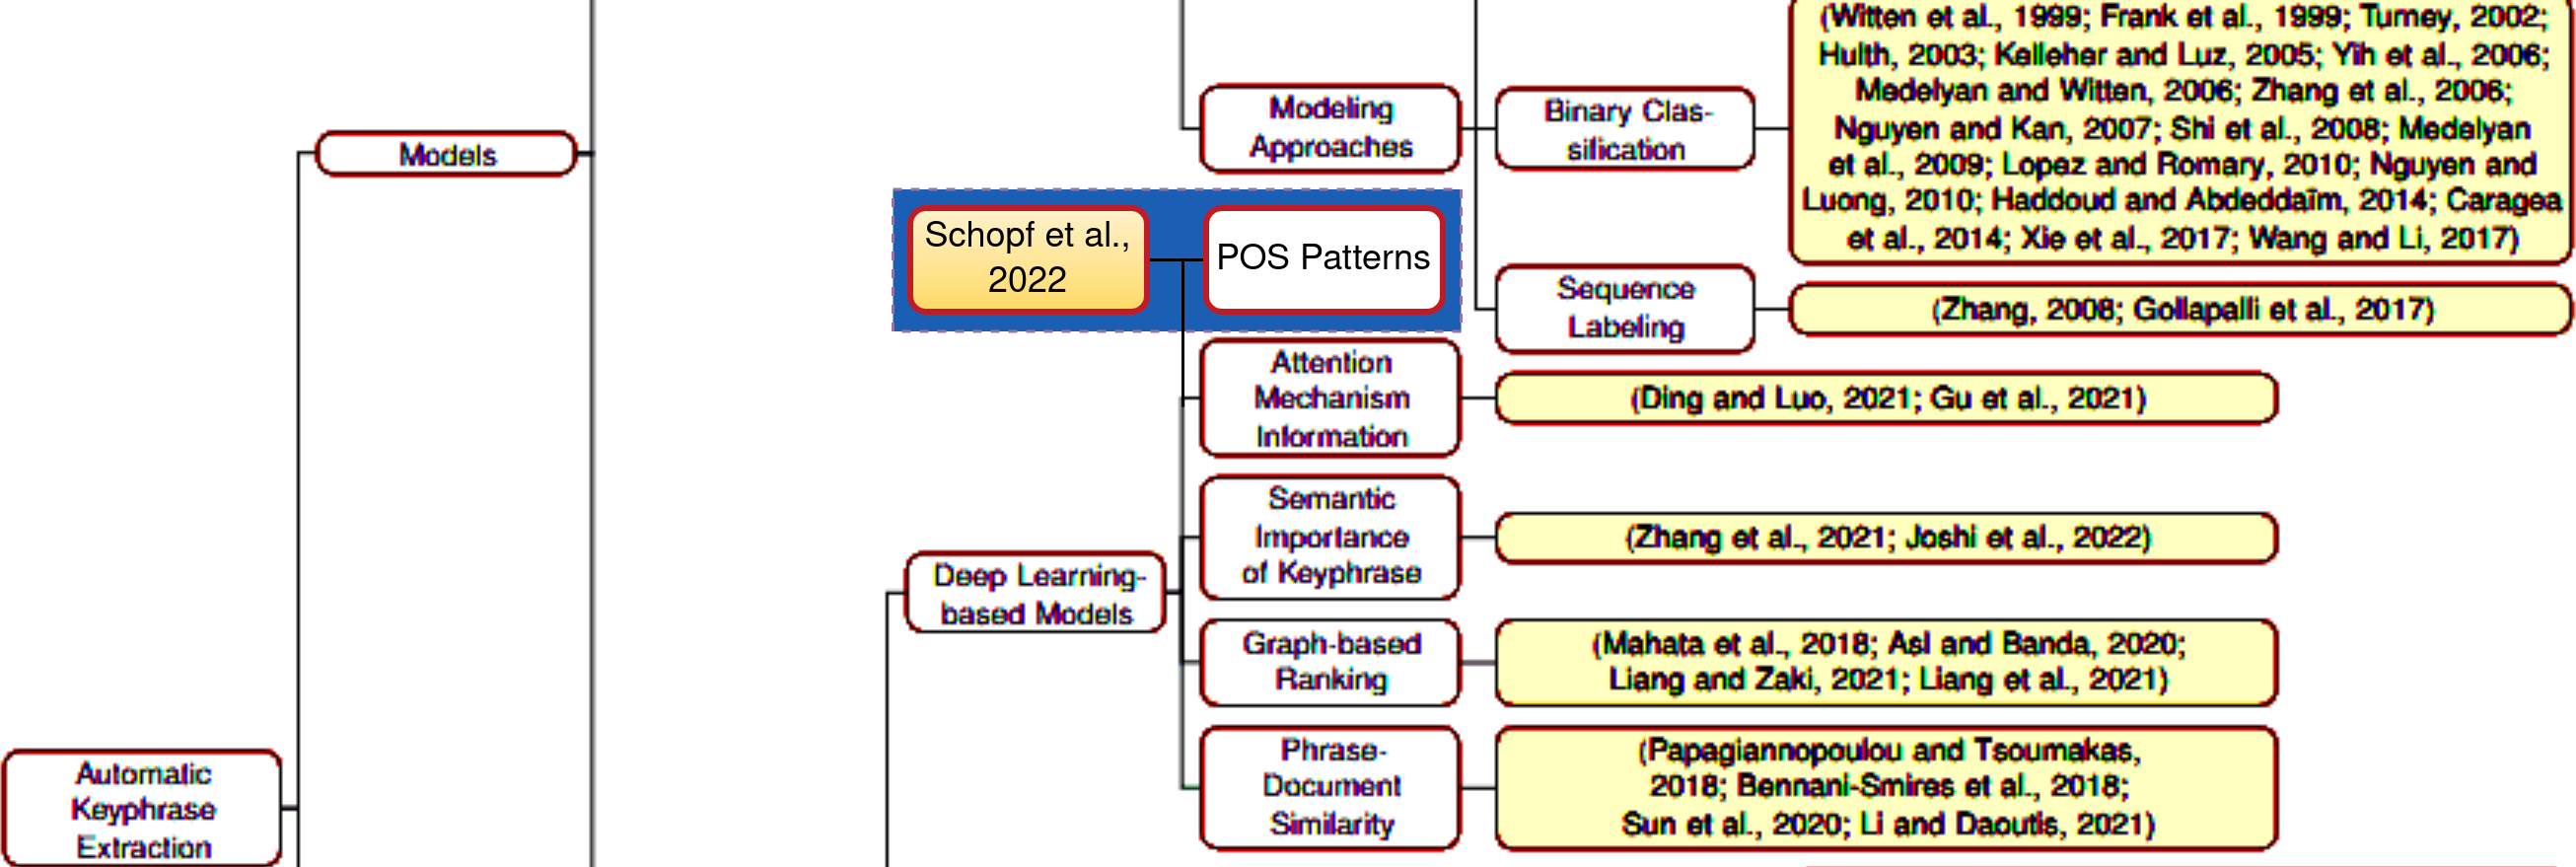
\includegraphics[width=110mm,scale=0.5]{pic/sota_lm_adapte.png}
    \caption{Extrait de l'état de l'art sur l'extraction des mots-clés, adapté de \citet{xie2023}}
    \label{fig:enter-label}
\end{figure}
\notecite{schopf2022}
\end{frame}

\begin{frame}{Fonctionnement de la méthode \textit{PatternRank}}
%\begin{itemize}
%\item extraction des phrases-clés non-supervisée
%\item exploite des modèles de langues pré-entraînés + parties du discours
%\end{itemize}
\begin{enumerate}[<+->]
\item entrée : un seul document texte tokenisé
\item étiquetage des tokens avec les balises POS
\item sélection des phrases-clés candidates correspondant au modèle POS 
\item génération des plongements du document et des phrases-clés candidates par un modèle de langue
\item calcul des similarités cosinus entre les plongements du document et des phrases-clés candidates + classement des phrases-clés
\item extraction des \textit{N} phrases-clés les plus représentatives
\end{enumerate}
\begin{figure}
    \centering
    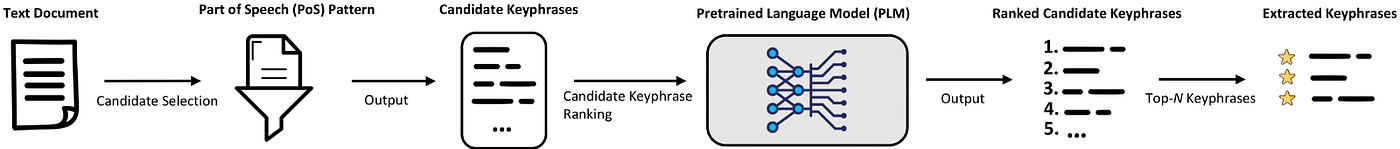
\includegraphics[width=110mm,scale=0.5]{pic/patternrank_workflow.png}
    \caption{\textit{Workflow} de la méthode \textit{PatternRank} \citep{schopf2022}.}
    \label{fig:enter-label}
\end{figure}
\end{frame}

\begin{frame}{Liste des phrases-clés avec \texttt{keyphrase-vectorizers}}
%\begin{table}
%\begin{tabular}{l|r}
%\small
%\rowcolor[HTML]{FFCCC9} 
%\textsc{\textbf{Phrase-clé}} & \cellcolor[HTML]{DAE8FC}\textsc{\textbf{Score}} \\ \hline
%paroi épaissie & 0.9276 \\
%histologie fine & 0.9193 \\
%tissu gingival & 0.9179 \\
%21c leçon & 0.9162 \\
%travaux récents & 0.9152 \\
%entrecroisement dos pyramides & 0.9145 \\
%érysipèle périodique annuel & 0.9135 \\
%cicatriciel & 0.9118 \\
%fibromes & 0.9109 \\
%affeclions & 0.9091
%\end{tabular}
%\caption{Liste des dix phrases-clés les plus pertinentes selon \texttt{keyphrase-vectorizers}.}
%\end{table}
\begin{table}[!htb]
\footnotesize
    \begin{minipage}{.5\linewidth}
      \centering
        \begin{tabular}{l|r}
         \rowcolor[HTML]{FFCCC9} 
\textsc{\textbf{Phrase-clé}} & \cellcolor[HTML]{DAE8FC}\textsc{\textbf{Score}} \\ \hline
            paroi épaissie & 0.9276 \\
			histologie fine & 0.9193 \\
			tissu gingival & 0.9179 \\
			21c leçon & 0.9162 \\
			travaux récents & 0.9152 \\
			entrecroisement dos pyramides & 0.9145 \\
			érysipèle périodique annuel & 0.9135 \\
			cicatriciel & 0.9118 \\
			fibromes & 0.9109 \\
			affeclions & 0.9091
        \end{tabular}
        \subcaption{Corpus \og{}Charcot\fg{}.}
    \end{minipage}%
    \begin{minipage}{.5\linewidth}
      \centering
        \begin{tabular}{l|r}
         \rowcolor[HTML]{FFCCC9} 
\textsc{\textbf{Phrase-clé}} & \cellcolor[HTML]{DAE8FC}\textsc{\textbf{Score}} \\ \hline
            trois lieues loing & 0.9369 \\
			detfeins pernicieux & 0.9292 \\
			21 mat & 0.9289 \\
			attaques syncopales2 & 0.9278 \\
			accufoit & 0.9255 \\
			diapason cataleptise & 0.9252 \\
			membre faidt & 0.9245 \\
			anes & 0.9242 \\
			toutesfois & 0.9235 \\
			demi culbute & 0.9217
        \end{tabular}
        \subcaption{Corpus \og{}Autres\fg{}.}
    \end{minipage} 
      \caption{Liste des dix phrases-clés les plus pertinentes selon \texttt{keyphrase-vectorizers} dans les deux corpus.}
\end{table}
\end{frame}

\begin{frame}{Utilisation des librairies \texttt{keybert} et \texttt{keyphrase-vectorizers}}
Ressources en ligne : \pause
\begin{itemize}[<+->]
\item \href{https://colab.research.google.com/drive/1sBJP-lJcKZPgIqWzFRNfrBn3domuy1tP?usp=sharing}{Lien Google Colab}\\
pré-requis :
\begin{itemize}[<+->]
\item bonne connexion Internet
\item mémoire RAM suffisante
\end{itemize}
\item \href{https://github.com/ljpetkovic/Charcot\_KeyBERT\_Keyphrase-Vectorizers?tab=readme-ov-file}{Dépôt GitHub}
\end{itemize}

\end{frame}

\begin{frame}{Passage à l'échelle}
\pause
Pour traiter de grands corpus, il existe la possibilité de demander l'accès à la plateforme technologique \href{https://sacado.sorbonne-universite.fr/}{\textsc{MeSU}}, hébergée par \textsc{SACADO} (Service d’Aide au Calcul et à l’Analyse de Données).\pause
\bigskip

Elle est composée d’un supercalculateur, d’un environnement de virtualisation et d’un système de stockage de données.
\end{frame}

